%\subsection{Dimensionnement d'un amplificateur à transistor }
%\vspace{1cm}
Soit le circuit suivant :
%\vspace{1cm}
%\begin{center}
%\includegraphics[width=12cm]{ampli_transistor2.png}
%\end{center}
%	\begin{center}
%			%\includegraphics[width=8cm]{}
%			\begin{circuitikz}[scale=0.8]\draw
%			(0,1) to [short,o-] (6,1)
%			%(4,6) to [short] (9,6)
%			(0,3) node[anchor=east] {In} to [short,o-] (1,3)
%			(0,2.7) to [open, v_=$V_{in}$]  (0,1.2)
%			(1,3) to [C=$C_{in}$ ](1.5,3)
%			(1.5,3) to [short,-*] (2,3)
%	%
%			(2,6) node[alimp ] (alim) {}
%			(alim.text) node {$+V_{dc}$}
%	%		
%			(2,3) to [R, l_=$R_{b1}$](2,6)
%			%(2,3) to [R=$R_{b2}$](2,1)
%	%		
%			(4,3) node[nigfetec] (mos) {}
%			%(mos.B) node[anchor=west] {B}
%			(mos.G) to [short] (2,3)
%	%		
%			(mos.D) to (4,4) to [R, l_=$R_D$] (4, 6)		
%			%(4,5.5) to [R] (mos.D)
%	%		
%			(mos.D) to [short,-*](4,3.5)  to [short] (4.25,3.5)
%	%		
%			(mos.S) to [short] (4,1)% to [short, -o](2,0)  node[anchor=west] {S}
%	%		
%			(4.25,3.5) to [C, l^=$C_{out}$] (6,3.5) to  [short](6,3.5) to [short,-o](6.5,3.5)node [anchor=south] {Out}	
%			(6,3.5) to [generic, l_=$R_{ch}$] (6,1)
%			(6.5,3.5) to [open,v^=$V_{out}$] (6.5,1)
%	%		
%			(4,6) node[alimp ] (alim2) {}
%			(alim2.text) node {$E$}
%			
%			 (4,1) node[ground] {} to  [short, -*] (4,1)
%		%	(9,1) to [battery, l_=$E$](9,6)
%	%		%(1,0) to [short, -o](-1,0)  node[anchor=east] {S}
%	%		
%	%%			(0,0) node[anchor=east] {In} 
%	%%			to [short, o-] (1,0) 
%	%%			to [open, v=$V_{GS}$] (1,-2)
%	%%			to [short, -o] (0,-2)
%	%%			to  (0,-2) node[anchor=east] {S}
%	%%			to [short] (3,-2)
%	%%			(3,0) to [cI=$ g_m \cdot V_{GS}$] (3,-2)
%	%%			(3,-2) to [short, -o] (4,-2) node[anchor=west] {S}
%	%%			(3,0) to [short, -o] (4,0)
%	%%			to node[anchor=west] {D} (4,0)
%	%	%		
%			;\end{circuitikz}
%		\end{center}
\begin{center}
			%\includegraphics[width=8cm]{}
			\begin{circuitikz}[scale=1]\draw
			(0,1) to [short,o-] (9,1)
			(4,6) to [short] (9,6)
			(0,3) node[anchor=east] {In} to [short,o-] (1,3)
			(0,3) to [open, v_<=$V_{in}$]  (0,1)
			(1,3) to [C=$C_{in}$ ](1.5,3)
			(1.5,3) to [short,-*] (2,3)
	%
			(2,6) node[anchor=south ] (alim) {$+V_{DC}$}
			(1.6,6) -- (2.4,6) %bar under the label
			%(alim.text) node {}
	%		
			(2,3) to [R, l_=$R_{B1}$](2,6)
			%(2,3) to [R=$R_{B2}$](2,1)
	%		
			(4,3) node[nfet] (mos) {}
			%(mos.B) node[anchor=west] {B}
			(mos.G) to [short] (2,3)
	%		
			(mos.D) to (4,4) to [R, l_=$R_D$] (4, 6)		
			%(4,5.5) to [R] (mos.D)
	%		
			(mos.D) to [short,-*](4,3.5)  to [short] (4.25,3.5)
	%		
			(mos.S) to [short] (4,1)% to [short, -o](2,0)  node[anchor=west] {S}
			(mos.S) -- (mos.B) %source to bulk connection		
	
			(4.25,3.5) to [C, l^=$C{out}$] (6,3.5) to  [short](6,3.5) to [short,-o](6.5,3.5)node [anchor=south] {Out}	
			(6,3.5) to [generic, l_=$Z_{ch}$] (6,1)
			(6.5,3.5) to [open,v^<=$V_{out}$] (6.5,1)
	%		
			(9,6) to [battery, l=$E$](9,1)
	%		%(1,0) to [short, -o](-1,0)  node[anchor=east] {S}
	%		
	%%			(0,0) node[anchor=east] {In} 
	%%			to [short, o-] (1,0) 
	%%			to [open, v=$V_{GS}$] (1,-2)
	%%			to [short, -o] (0,-2)
	%%			to  (0,-2) node[anchor=east] {S}
	%%			to [short] (3,-2)
	%%			(3,0) to [cI=$ g_m \cdot V_{GS}$] (3,-2)
	%%			(3,-2) to [short, -o] (4,-2) node[anchor=west] {S}
	%%			(3,0) to [short, -o] (4,0)
	%%			to node[anchor=west] {D} (4,0)
	%	%		
			;\end{circuitikz}
	\end{center}
%\vspace{1cm}
Où $E=12V$, $R_{B1}=100k\Omega$ et $R_D=200\Omega$.\\

Cet étage amplificateur doit permettre de mesurer à sa sortie une tension $v_{out}(t)$ égale au signal utile d'entrée $v_{in}(t)$ multiplié par un gain $A_v$.\\

Les capacités d'entrée $C_{in}$ et de sortie $C_{out}$ se comportent comme des courts-circuits pour les signaux utiles.\\

Les courbes caractéristiques du transistor MOS utilisé sont fournies à la page suivante.
%\newpage
%\begin{center}
%\vspace*{-2cm}
%\hspace*{-0.8cm}
%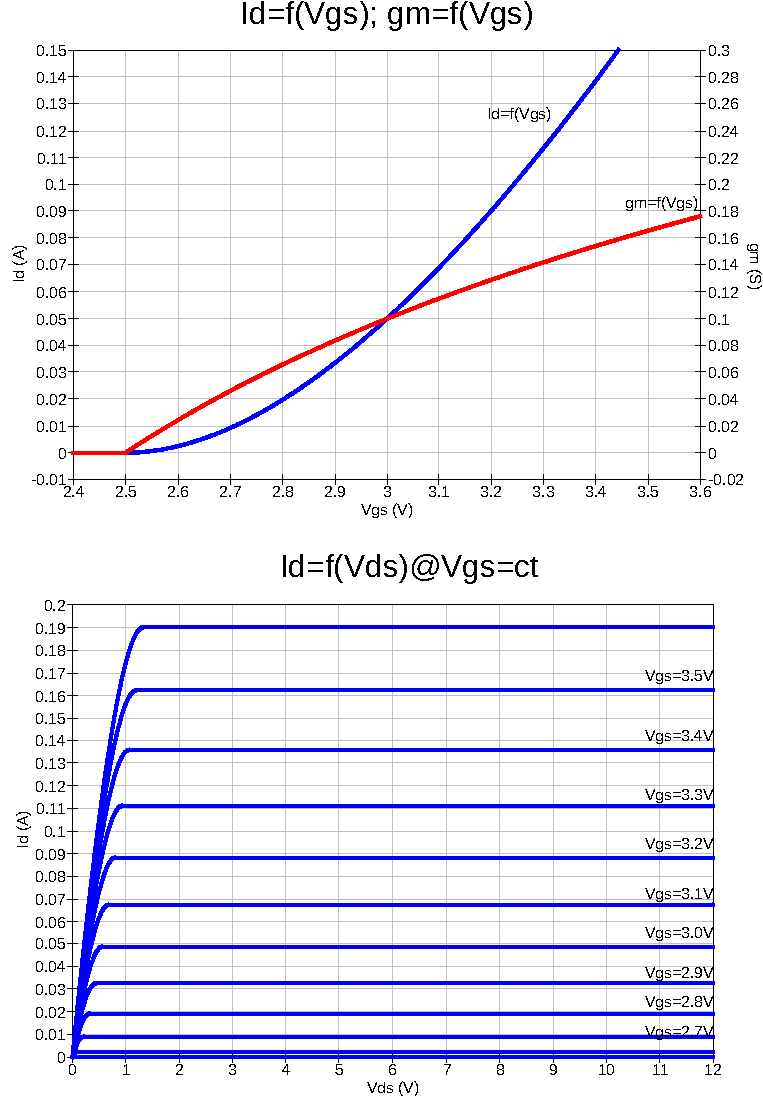
\includegraphics[width=17cm]{courbes_mos-crop.pdf}
%\end{center}

%QUESTION 1.
\Question
{
%question
%\textbf{
Sur base des courbes fournies, dimensionner la tension de polarisation $V_{dc}$ afin que l'étage amplificateur de tension ait un gain à vide $A_v=28.3dB$. 

%\\
%}
}
{%R
%-\\
\begin{enumerate}

	
	\item \fbox{$G=28.3dB$}\\
	
	Donc le gain en tension $A_v=\frac{V_{out}}{V_{in}}=\pm 10^{G/20}\approx \pm26$\\
	
	Or, on connaît le gain de cet étage à vide lorsqu'il est polarisé correctement :
	$V_{out}=-g_m R_D V_{in}$ 	
	
	d'où:	$A_v=-g_m R_D$
	
	Et on obtient donc la transconductance:
	$g_m=-\frac{A_v}{R_D}=\frac{-(-26)}{200\Omega}=0.13 S$
	
	\item \fbox{Courbe de transfert du transistor}\\
	
	On impose donc $g_m=0.13S$.\\
	Via la caractéristique de transfert $I_D=f(V_{GS})$ (et donc $g_m=f(V_{GS})$), on trouve $V_{GS}$.\\
%	\begin{center}
%		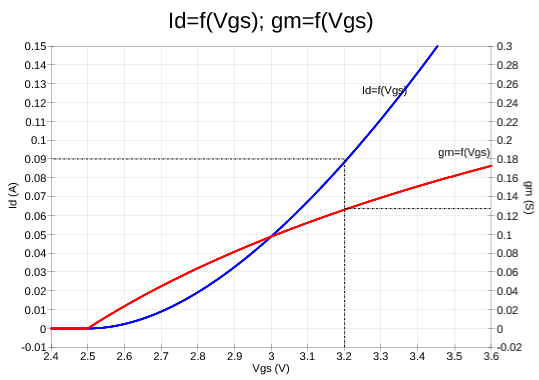
\includegraphics[width=10cm]{caract_mos_cor1.png}
%	\end{center}
	~\\
Selon la caractéristique, on a:\\
	$V_{GS}\cong 2.84V$\\
		
La tension de polarisation à la grille est:\\
	$V_{GS}=V_{DC}$ (pas de courant continu dans la résistance)\\
	
%De plus,\\
%	$V_{GSQ}=V_{GQ}-V_S=V_{GQ}+V_{CC}=V_{R2}$
%	
%Le diviseur résistif nous donne:\\
%	$V_{GSQ}=V_{R2}=\frac{R_2}{R_1+R_2}\left(V_{pol}-\left(-V_{CC}\right)\right)$\\
%	
%Donc:\\
%	$V_{pol}=\frac{R_1+R_2}{R_2}V_{GSQ}-V_{CC}=\frac{2R_2+R_2}{R_2}V_{GSQ}-V_{CC}$\\
	$\Rightarrow$ \fbox{$V_{DC}=2.84V$}
	
\end{enumerate}
}

%\Questiontsuite{Question 2.1. suite}{10cm}{8}
%{}
%{
%
%}

%\Questiontsuite{Question 2.1. suite}{8cm}{}
%{}
%{
%~\\
%Selon la caractéristique, on a :\\
%	$V_{GSQ}\cong 3.2V$\\
%	
%	Le diviseur résistif nous donne le potentiel de polarisation à la grille:\\
%	$V_{GQ}=\frac{R_2}{R_1+R_2}V_{pol}=\frac{R_2}{2R_2+R_2}V_{pol}=\frac{1}{3}V_{pol}$\\
%	
%	Avec:\\
%	$V_{GSQ}=V_{GQ}-V_S=V_{GQ}+V_{CC} \Leftrightarrow V_{GQ}=V_{GSQ}-V_{CC}=3,2-12=-8,8V$
%	
%	$\Rightarrow$ \fbox{$V_{pol}=3V_{GQ}=3*(-8,8)=-26,4V$}\\
%}

%QUESTION 2.
\Question
{%question
%\textbf{
Calculer la puissance dissipée par le transistor, due à la polarisation.

%}
}
{
~\\
\underline{\textbf{METHODE 1:}}\\

$V_{DS}=E-R_D\cdot I_{D}$\\
 
$P_{T}=V_{DS}\cdot I_{D}=\left(E-R_D\cdot I_{D}\right)I_{D}=E\cdot I_{D}-R_D\cdot I_{D}^2$\\
	
On connait la tension $V_{GS}=2.84V$. La caractéristique de transfert du transistor nous donne $I_{D}=25mA$ (voir page précédente).\\

$\Rightarrow$ \fbox{$P_{T}=E\cdot I_{D}-R_D\cdot I_{D}^2=175mW$}\\

\underline{\textbf{METHODE 2:}}\\

La réponse à la question précédente nous donne $V_{DS}=7V$.\\
$\Rightarrow$ \fbox{$P_{T}=V_{DS}\cdot I_{D}=7\times 0.025=175mW$}

}




%QUESTION 3.
\Question
{%question
%\textbf{
Vérifiez que le transistor reste bien dans sa zone de pincement si on impose à l'entrée de l'étage amplificateur une tension dont l'amplitude est bornée entre $-0.1V$ et $0.1V$.

}
{
~\\
Exprimons cette tension d'entrée comme suit :
$$v_{in}(t)=V_{in}\cdot fct(t)=\pm 0.1\cdot fct(t)$$

La tension de sortie sera donc comprise entre $-2.6V$ et $2.6V$ :
$$v_{out}(t)=V_{out}\cdot fct(t)=A_v\cdot v_{in}(t)= \pm 2.6\cdot fct(t)$$


On a donc une tension grille-source :
$$V_{GS}=V_{GS} + v_{gs}=V_{DC} + v_{in}(t)=2.84\pm 0.1\cdot fct(t)$$

Et une tension drain-source de polarisation :
$$V_{DS}=E-R_D\cdot I_{D}=7V$$

Ce qui nous donne le point de fonctionnement de la caractéristique de sortie du transistor $(I_{D};V_{DS})=(25mA;7V)$

De plus, l'équation suivante $V_{DS}=E-R_D\cdot I_{D}$ nous permet de trouver la droite de charge  passant par le point de fonctionnement:\\
$$I_D=-\frac{1}{R_D}V_{DS}+\frac{E}{R_D}=-0.005V_{DS}+60mA$$

En superposant cette droite de charge à la caractéristique de sortie, on voit que le dimensionnement convient puisqu'en zone de pincement, on dispose d'une excursion allant de $0.5V$ à $12V$ alors que le signal de sortie est compris entre $V_{DS}-2.6V$ et $V_{DS}+2.6V$.
\begin{center}
	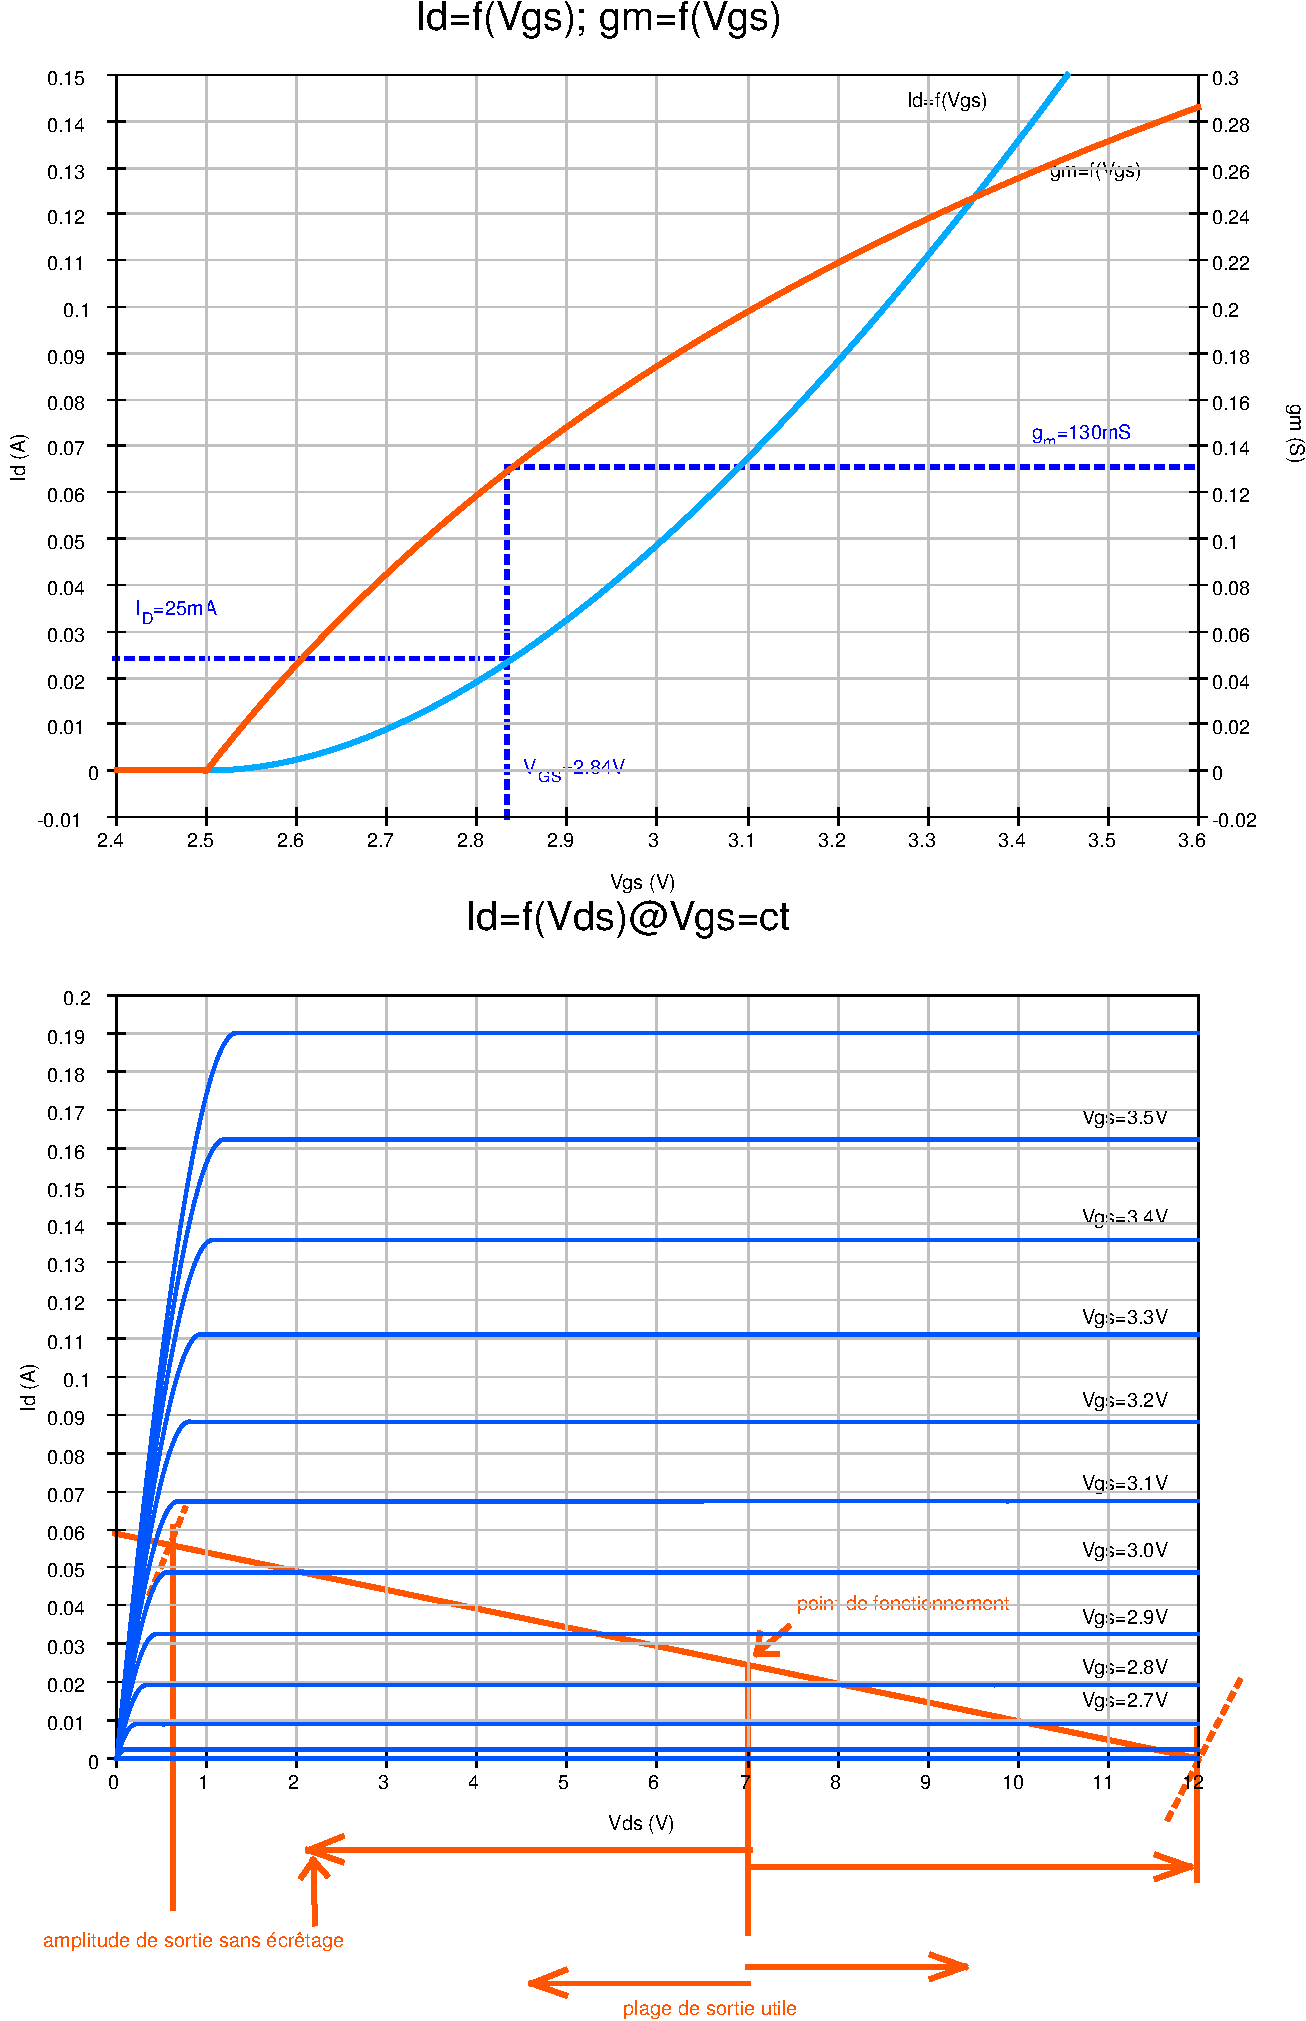
\includegraphics[width=10cm]{mos_exam_corr-crop.pdf}
%	\vspace{-5cm}
\end{center}
}
%\vspace*{-1cm}
%\newpage
\begin{center}
%\vspace*{-1cm}
%\hspace*{-0.8cm}
\ifgv{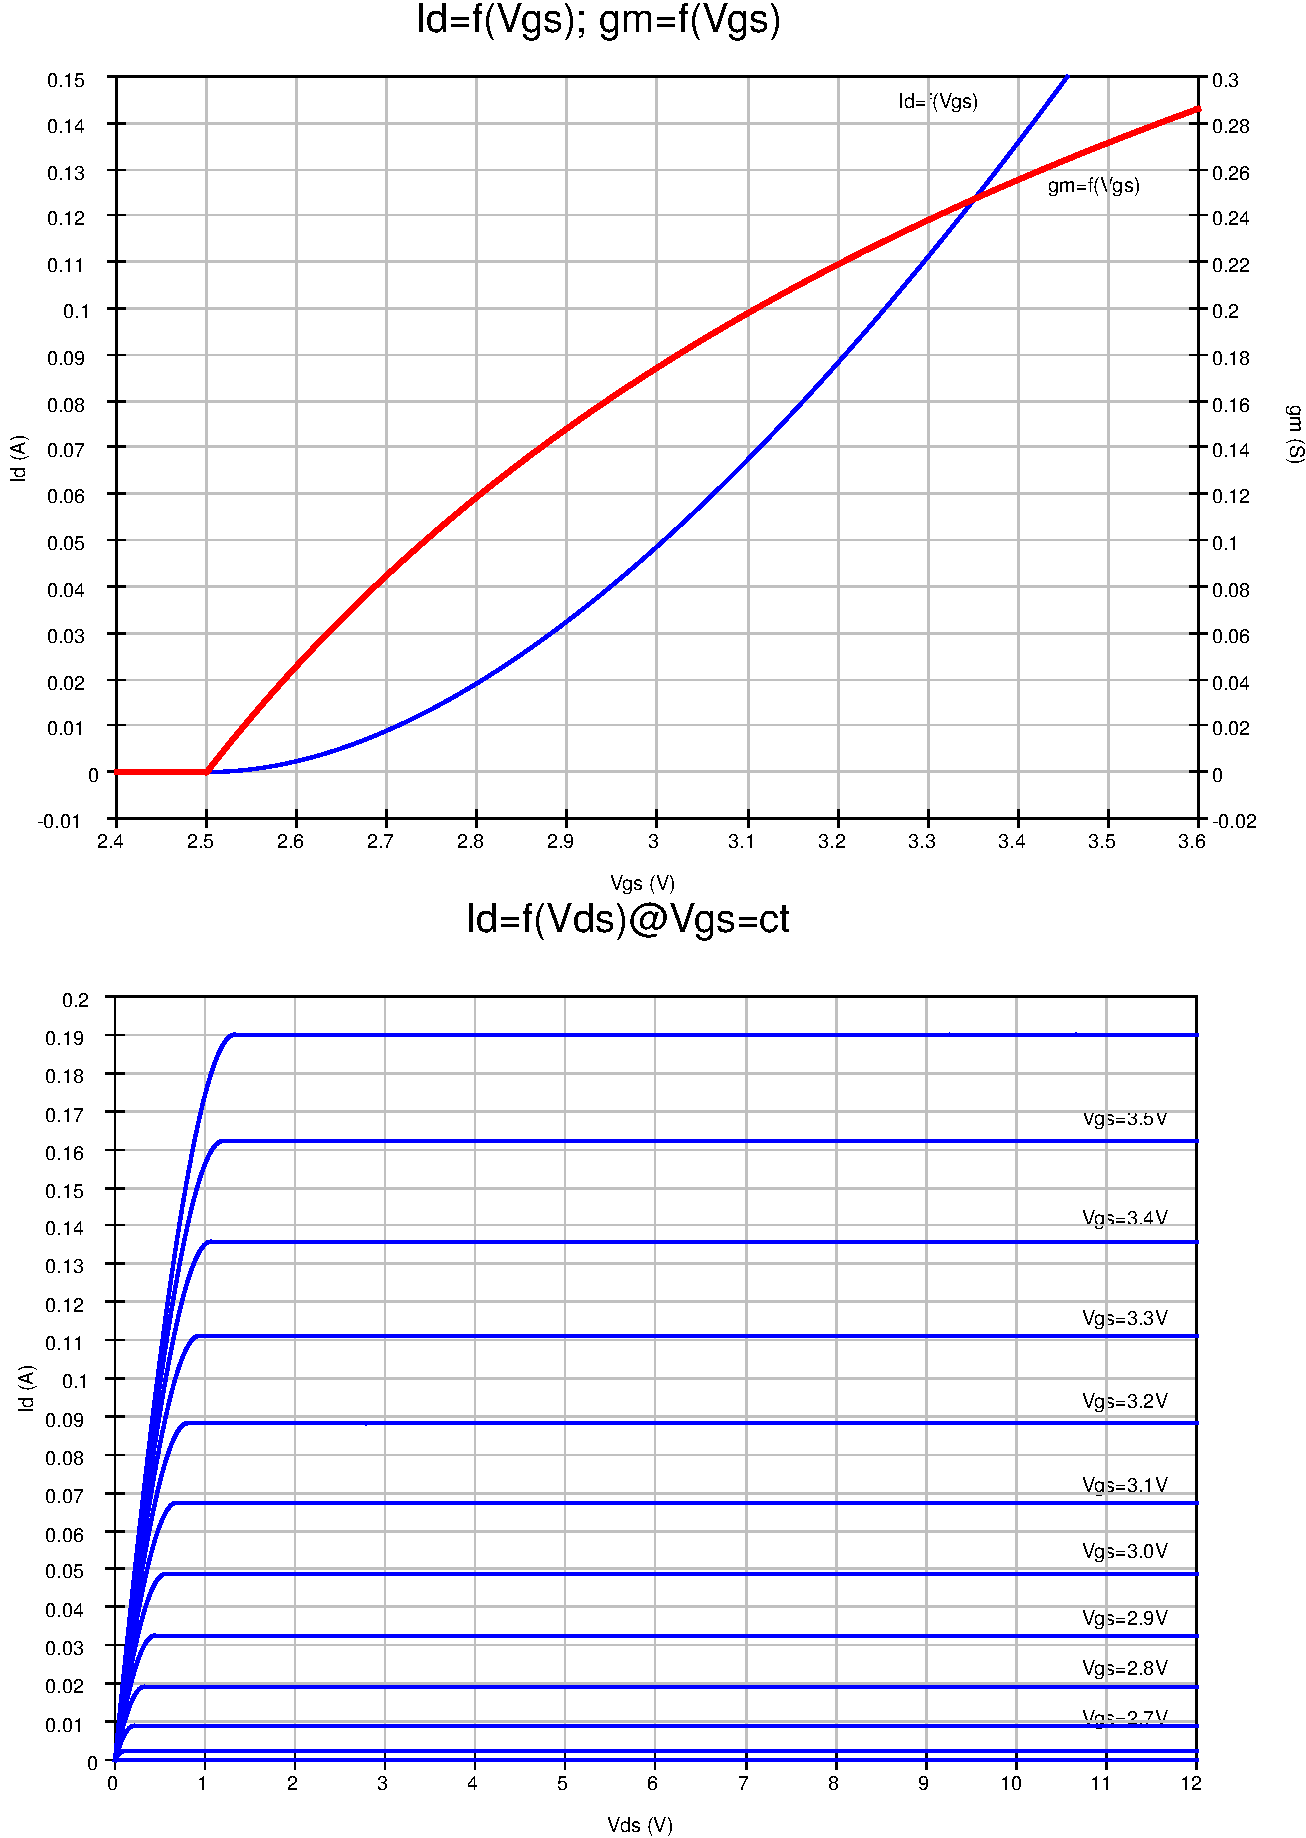
\includegraphics[width=16cm]{courbes_mos_2k16-crop.pdf}}
%\vspace*{-5cm}
\end{center}